%!TEX root = ../main.tex
\chapter{Univent Design}
\label{chap:design}
\section{Overview}

The app design is a very important phase of the development lifecycle, as it can have an impact whether or not the app is accepted by the users. This chapter presents the choices made for the design of the aplication.

\section{Android Application Design}
\label{android app design}
The user interface is designed using widgets. Android provides  basic widgets such as, image view, textview, etc., which can be used to create the application. All these widgets are incuded in the Android SDK. Android gives users the possibility to create their own widgets, named custom widgets.

All the screens in the project are composed of various widgets, both basic and customized. 

The home screen, includes widgets such as, RecycleView, TextView, ImageView. The recycleview is populated with data directly from the database.
\begin{itemize}
	\item \textbf{TextView} - 
	A textview displays text to the user, normally displaying contextual information or the name of other elements on the screen. Figure \ref{fib:textview}, shows how to define a text view in the XML editor.	
\begin{figure}[!htbp]
		\centering
		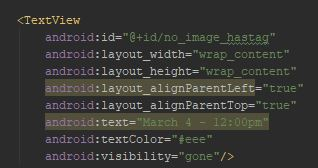
\includegraphics[width=0.23\textheight]{textview}	
		\caption{Define a TextView in XML}
		\label{fib:textview}
\end{figure}

\item \textbf{ImageView} - 
 	An Imageview is used to display image to the user from the resource file or from an external source, like the internet.	
 	The following snippet is an example of imageview, refer to figure \ref{fib:imageview}
 	
\begin{figure}[h]
 				\centering
 		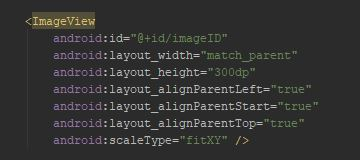
\includegraphics[width=0.45\textheight]{imageview}	
 		\caption{Define a ImageView in XML}
 		\label{fib:imageview}
\end{figure}
 \item \textbf{RecycleView} - 
According to the official android website, \say{a Recycleview is a view group that displays a list of scrollable items}. The list items are automatically inserted to the list using an Adapter that pulls content from a source such as an array or database query and converts each item result into a view that's placed into the list.
Figure \ref{fig:xmlrecycleview}, shows how to declare a recycle view.
\begin{figure}[h]
	\centering       
		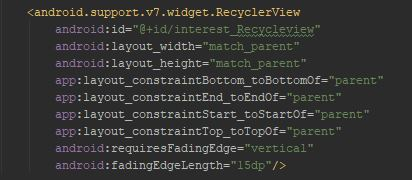
\includegraphics[width=0.45\textheight,natwidth=610,natheight=300]{recycleview}
		\caption{Defining RecycleView}
		\label{fig:xmlrecycleview}	
\end{figure} 

Recycleviews are normally accompanied with cardveiws, these shows information inside cards, and its corners can be customized by the user. The main function of these cards is to act as the rows of the recycleview.
	
\item \textbf{ViewPager - } 
A viewPager is viewgroup that allows the user to swipe left or right to display a new screen. Its a more efficient and user friendly way of displaying screens to users, refer to Appendix \ref{screen_design}.
\end{itemize} 
\pagebreak
\section{Initial Design}
Before the final design of the app was created, various designs were made in attempt to give a better UI experience to the user, refer to Appendix \ref{screen_design}. All the designs were made with the Android XML editor to see exactly how it will look on a mobile device. Using the XML editor made designing simple, meaning no need of wireframe designs before recreating them for the app, which saved a lot of time. All the widgets mentioned above in section \ref{android app design}, were used to complete the design.
Extensive research on similar applications, section \ref{similar_app}, provided inspiration for the final look of the app and the meeting with the client also provided ideas for new features to implement. 
The app was further redesigned to be more user friendly, with two new screens created, Discover and Interest(named as "for you" in the app), using viewpager, as detailed in \ref{android app design}, so users can swipe left or right to move between  screens as shown below in figure \ref{fig:homescreen}.

\begin{figure}[h]
	\centering       
	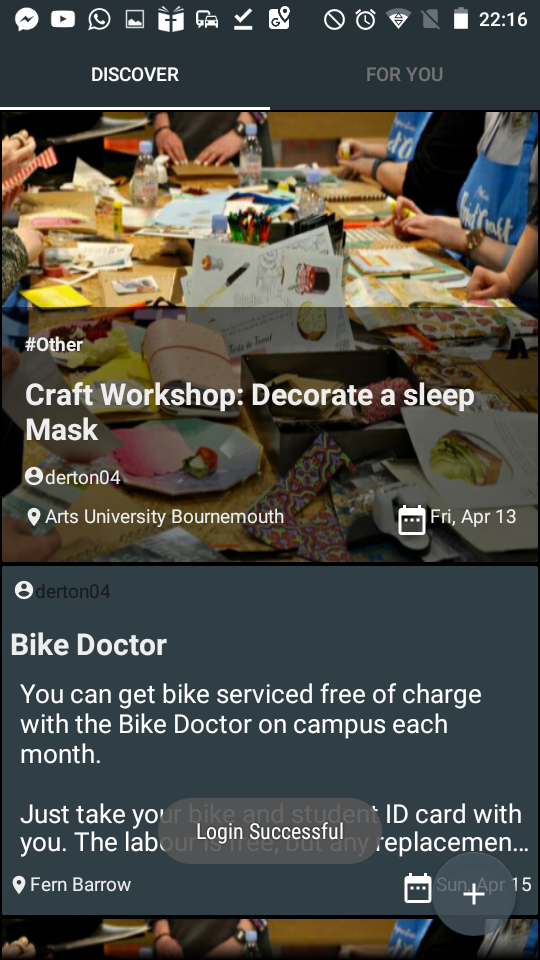
\includegraphics[width=0.25\textheight]{discover}
	\caption{Home Screen}
	\label{fig:homescreen}	
\end{figure}

The discover screen shows all the upcoming events with no filter, while the "for you" screen  shows only recommended events based on the user interest. In order to achieve this a new feature was to be added, as a way for the user to choose what they were into. A snippet of the Interest screen can be found in Appendix \ref{screen_design}.

\section{Database Design}
Figure \ref{fig:database_design}, describes the structure of the database. The event table contains all the information of the event, the user table has all the user information and finally the GoingTable, contains the ID of the users an the specific event ID the wish to attend.
\begin{figure}[h!]
	\centering       
	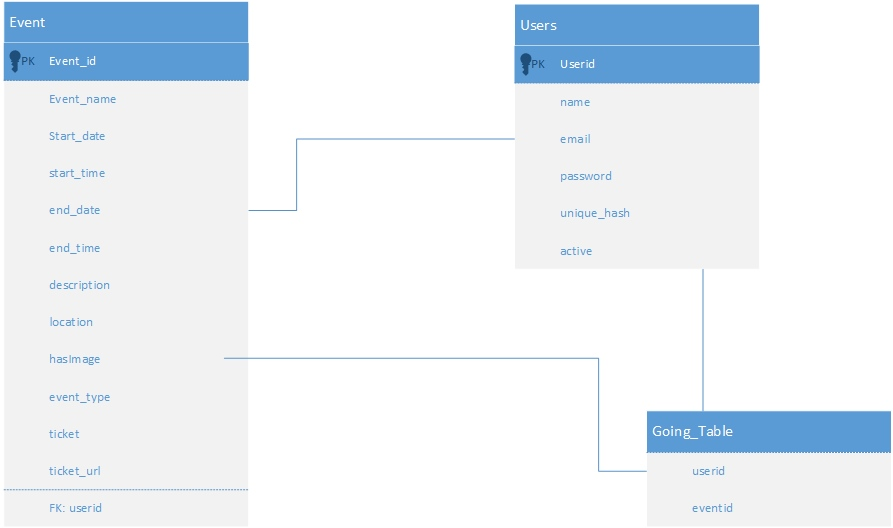
\includegraphics[width=0.6\textheight]{database_design}
	\caption{Database Design}
	\label{fig:database_design}	
\end{figure}
\subsection{Security}
 Considering the importance of data it is not a surprise for attackers to target the data these are containing. In this section various challenges in database security are discussed.
\begin{itemize}	
\item 	\textbf{Blank Password, blank email:} In order to avoid this issue, a password and email validation has been put in place, which will notify the user if any of the fields are left blank.

\item 	\textbf{Secure credential:} User passwords are not stored directly onto the database, but are encrypted using a  hash key. The hash key is then stored in the database, whenever the password is called it is then decoded.
	
\item 	\textbf{Excessive privileges:} Granting  Users (or applications) database privileges that exceed the requirements of their task, these privileges may be abused for malicious actions. 
	
\item 	\textbf{Weak Authentication:} Weak authentication allows attackers to take the identity of database users. A counter measure for this issue will be to Implement a two-factor authentication.
\end{itemize}

\subsection{General Architecture }
An Android device with the Univent application already installed communicates with the web service using a RESTful API.
The application sends HTTP requests with GET/POST method headers and receives formatted JSON responses. The API is written in PHP and handles querying the MYSQL database. Figure \ref{fig:API_design}, shows the system architecture.
\begin{figure}[h!]
	\centering       
	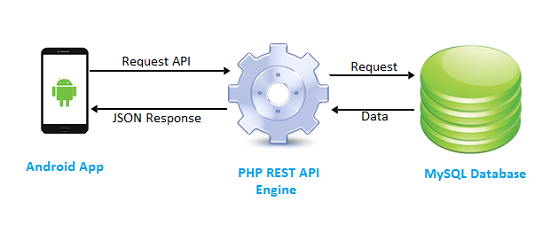
\includegraphics[width=0.5\textheight]{php-mysql-rest-api-for-android}
	\caption{Rest API}
	\label{fig:API_design}	
\end{figure}
\FloatBarrier




